\documentclass{report}
\usepackage[utf8]{inputenc}
\usepackage[T1]{fontenc}
\usepackage{geometry}
\geometry{a4paper, margin=1in}
\usepackage{graphicx}
\usepackage{amsmath}
\usepackage{amsfonts}
\usepackage{amssymb}
\usepackage{listings}
\usepackage{xcolor}
\usepackage{hyperref}
\usepackage{float}
\usepackage{caption}
\usepackage{subcaption}

% ====== COULEURS DU THEME : GOLDEN GLOW + SOFT ESPRESSO ======
\definecolor{GoldenGlow}{RGB}{212,175,55}
\definecolor{SoftEspresso}{RGB}{62,39,35}
\definecolor{LightCream}{RGB}{255,253,245}
\definecolor{AccentGray}{RGB}{120,110,100}
\definecolor{CodeBg}{RGB}{248,246,240}
\definecolor{CodeKeyword}{RGB}{62,39,35}
\definecolor{CodeComment}{RGB}{120,110,100}
\definecolor{CodeString}{RGB}{170,140,40}

% ====== STYLE DES LEGENDES DES FIGURES ======
\captionsetup{
  labelfont={bf,color=SoftEspresso},
  textfont={it,color=AccentGray},
  labelsep=period
}

\hypersetup{
    colorlinks=true,
    linkcolor=SoftEspresso,
    filecolor=GoldenGlow,
    urlcolor=GoldenGlow,
    citecolor=SoftEspresso
}

\lstdefinestyle{mystyle}{
    backgroundcolor=\color{CodeBg},
    commentstyle=\color{CodeComment}\itshape,
    keywordstyle=\color{CodeKeyword}\bfseries,
    numberstyle=\tiny\color{AccentGray},
    stringstyle=\color{CodeString},
    basicstyle=\ttfamily\footnotesize\color{SoftEspresso},
    breakatwhitespace=false,
    breaklines=true,
    captionpos=b,
    keepspaces=true,
    numbers=left,
    numbersep=5pt,
    showspaces=false,
    showstringspaces=false,
    showtabs=false,
    tabsize=2,
    frame=single,
    framerule=0.6pt,
    rulecolor=\color{GoldenGlow}
}

\lstset{style=mystyle}
\usepackage{tikz}
\usepackage{setspace}

% ====== CHEMIN DES IMAGES ======
\graphicspath{{images/}{./}}

\begin{document}

\begin{titlepage}
\centering

\vspace*{0.5cm}

% ====== HEADER ======
{\large \textbf{\color{SoftEspresso}République Algérienne Démocratique et Populaire}}\\[0.2cm]
{\large \color{SoftEspresso}Ministère de l'Enseignement Supérieur et de la Recherche Scientifique}\\[0.5cm]

% ====== UNIVERSITY ======
{\Large \textbf{\textsc{\color{SoftEspresso}Université Ibn Khaldoun-Tiaret}}}\\[0.2cm]
{\large \color{SoftEspresso}Faculté d'Informatique}\\[0.8cm]

% ====== LOGO ======
\includegraphics[width=3.5cm]{logo.png}\\[0.8cm]

% ====== MAIN TITLE ======
{\color{GoldenGlow}\rule{\textwidth}{1.5pt}}\\[0.4cm]

{\Huge \textbf{\color{SoftEspresso}RAPPORT DE PROJET}}\\[0.2cm]
{\Huge \textbf{\color{SoftEspresso}DE FIN D'ÉTUDES}}\\[0.4cm]

{\color{GoldenGlow}\rule{\textwidth}{1.5pt}}\\[1cm]

% ====== SPECIALITY ======
{\large \textbf{\color{SoftEspresso}Spécialité :}}\\
{\Large \color{SoftEspresso}Ingénierie des Systèmes d'Information et Logiciel}\\[1cm]

% ====== PROJECT TITLE ======
{\color{GoldenGlow}\fbox{\color{black}
\parbox{0.9\textwidth}{
\centering
\vspace{0.3cm}
{\LARGE \textbf{\color{SoftEspresso}Authentification et Gestion des Rôles}}\\
\vspace{0.3cm}
}
}}\\[1.5cm]

% ====== STUDENTS ======
\begin{minipage}{0.45\textwidth}
\raggedright
\textbf{\large \color{SoftEspresso}Réalisé par :}\\[0.3cm]
\textbf{\color{GoldenGlow}\textbullet} \color{SoftEspresso}Ghoulam Mohamed Said\\
\textbf{\color{GoldenGlow}\textbullet} \color{SoftEspresso}Chelig Mohamed Amine\\
\textbf{\color{GoldenGlow}\textbullet} \color{SoftEspresso}Reddas Belkacem\\
\end{minipage}
\hfill
% ====== SUPERVISOR ======
\begin{minipage}{0.45\textwidth}
\raggedleft
\textbf{\large \color{SoftEspresso}Encadré par :}\\[0.3cm]
\textbf{\color{GoldenGlow}\textbullet} \color{SoftEspresso}Dr. Abdelkader Bougassa\\
\end{minipage}

\vfill

% ====== FOOTER ======
{\color{GoldenGlow}\rule{0.6\textwidth}{0.5pt}}\\[0.3cm]
{\large \textbf{\color{SoftEspresso}Année universitaire : 2025 - 2026}}

\end{titlepage}

\chapter{\color{SoftEspresso}Conception et Réalisation du Module d'Authentification et de Gestion des Rôles}

\section{\color{SoftEspresso}Présentation du Module}
L'authentification est le processus de vérification de l'identité d'un utilisateur. Dans le contexte d'une plateforme universitaire, où des données sensibles telles que les notes, les informations personnelles des étudiants et les contenus de cours sont stockées et manipulées, la mise en place d'un système d'authentification robuste est d'une importance capitale. Ce module a pour objectif de construire une barrière de sécurité fiable, garantissant que seuls les utilisateurs légitimes puissent accéder aux ressources qui leur sont autorisées, préservant ainsi l'intégrité, la confidentialité et la disponibilité des données du système.

\section{\color{SoftEspresso}Objectifs}
Les objectifs principaux de ce module sont les suivants :
\begin{itemize}
    \item \textbf{\color{SoftEspresso}Sécuriser l'accès :} Empêcher tout accès non autorisé aux différentes parties de l'application.
    \item \textbf{\color{SoftEspresso}Identifier les utilisateurs :} Fournir un mécanisme fiable pour identifier chaque utilisateur interagissant avec le système.
    \item \textbf{\color{SoftEspresso}Gérer les permissions :} Mettre en œuvre un contrôle d'accès basé sur les rôles (RBAC) pour différencier les permissions entre les différents types d'utilisateurs (administrateurs, enseignants, étudiants).
\end{itemize}

\section{\color{SoftEspresso}Fonctionnalités}
Pour atteindre ces objectifs, le module implémente les fonctionnalités suivantes :
\begin{itemize}
    \item \textbf{\color{SoftEspresso}Création de compte :} Permet aux nouveaux utilisateurs de s'inscrire. Ce processus est principalement géré par les administrateurs pour garantir un contrôle strict des accès.
    \item \textbf{\color{SoftEspresso}Connexion sécurisée :} Un formulaire de connexion où l'utilisateur fournit son email et son mot de passe. Le système valide ces informations pour accorder l'accès.
    \item \textbf{\color{SoftEspresso}Déconnexion :} Permet à un utilisateur de terminer sa session de manière sécurisée, en invalidant son jeton d'accès.
    \item \textbf{\color{SoftEspresso}Gestion des sessions (JWT) :} Utilisation des \textit{JSON Web Tokens} (JWT) pour gérer les sessions utilisateur. Après une connexion réussie, un jeton signé est généré et renvoyé au client. Ce jeton doit être inclus dans les en-têtes de chaque requête subséquente vers des routes protégées.
    \item \textbf{\color{SoftEspresso}Middleware de protection des routes :} Des intergiciels (\textit{middlewares}) sont mis en place sur le backend pour intercepter et valider le JWT de chaque requête entrante, protégeant ainsi les points d'accès de l'API.
    \item \textbf{\color{SoftEspresso}Gestion des rôles :} Le système définit plusieurs rôles, chacun avec un ensemble de permissions distinct :
    \begin{itemize}
        \item \textbf{\color{GoldenGlow}Admin :} Accès complet à toutes les fonctionnalités du système, y compris la gestion des utilisateurs et la configuration de la plateforme.
        \item \textbf{\color{GoldenGlow}Enseignant :} Accès aux fonctionnalités liées à la gestion de ses cours, à la notation de ses étudiants et à la communication.
        \item \textbf{\color{GoldenGlow}Étudiant :} Accès restreint à ses cours, ses notes et les informations le concernant.
        \item \textbf{\color{GoldenGlow}Guest (Invité) :} Rôle non authentifié avec des permissions minimales, généralement limité à la consultation de pages publiques.
    \end{itemize}
\end{itemize}

\section{\color{SoftEspresso}Contraintes}
Le développement de ce module a été guidé par plusieurs contraintes non fonctionnelles, essentielles pour la fiabilité du système :
\begin{itemize}
    \item \textbf{\color{SoftEspresso}Sécurité des données :} Les informations sensibles, en particulier les mots de passe, ne doivent jamais être stockées en clair. Le hachage robuste est une exigence absolue.
    \item \textbf{\color{SoftEspresso}Protection contre les attaques courantes :}
    \begin{itemize}
        \item \textbf{\color{SoftEspresso}Brute force :} Des mécanismes de limitation de débit (\textit{rate limiting}) doivent être en place pour prévenir les tentatives de connexion par force brute.
        \item \textbf{\color{SoftEspresso}IDOR (Insecure Direct Object References) :} Le système doit vérifier que l'utilisateur authentifié a bien le droit d'accéder à l'objet qu'il demande (par exemple, un étudiant ne peut pas voir les notes d'un autre étudiant en manipulant l'URL).
        \item \textbf{\color{SoftEspresso}Accès non autorisé :} Le contrôle d'accès basé sur les rôles doit être rigoureusement appliqué à chaque point d'accès de l'API.
    \end{itemize}
    \item \textbf{\color{SoftEspresso}Performance :} Le processus d'authentification et de vérification des permissions doit être optimisé pour ne pas introduire de latence perceptible pour l'utilisateur.
\end{itemize}

\section{\color{SoftEspresso}Conception}
\subsection{\color{SoftEspresso}Architecture}
L'architecture du module est répartie entre le client et le serveur :
\begin{itemize}
    \item \textbf{\color{SoftEspresso}Backend (Node.js avec Express) :} Gère la logique métier, l'interaction avec la base de données via l'ORM Prisma, la validation des informations d'identification, la génération des JWT et l'application des middlewares de sécurité.
    \item \textbf{\color{SoftEspresso}Frontend (React) :} Fournit l'interface utilisateur pour la connexion, l'inscription et la gestion des sessions. Il stocke le JWT de manière sécurisée (par exemple, dans un cookie HTTP-only) et l'envoie avec chaque requête à l'API.
\end{itemize}

\subsection{\color{SoftEspresso}Base de données}
La conception de la base de données, modélisée avec Prisma, est centrée autour des entités \texttt{User} et \texttt{Role}.
\begin{itemize}
    \item \textbf{\color{SoftEspresso}Table \texttt{User} :} Contient les informations sur les utilisateurs, telles que l'identifiant, le nom, l'email (unique), le mot de passe haché, et une clé étrangère \texttt{roleId} qui la lie à son rôle.
    \item \textbf{\color{SoftEspresso}Table \texttt{Role} :} Une table simple (ou une énumération dans notre cas) qui définit les rôles possibles dans le système (\texttt{ADMIN}, \texttt{ENSEIGNANT}, \texttt{ETUDIANT}).
\end{itemize}
La relation est de type "plusieurs-à-un" : plusieurs utilisateurs peuvent avoir le même rôle, mais un utilisateur n'a qu'un seul rôle.

\subsection{\color{SoftEspresso}Diagrammes UML (Description textuelle)}
\subsubsection{\color{SoftEspresso}Diagramme de classes}
\textit{Description du diagramme de classes :} Le diagramme de classes montrerait une classe \texttt{User} avec des attributs comme \texttt{id}, \texttt{email}, \texttt{passwordHash}, et des méthodes comme \texttt{login()}, \texttt{logout()}. Une énumération \texttt{Role} serait définie avec les valeurs \texttt{ADMIN}, \texttt{ENSEIGNANT}, \texttt{ETUDIANT}. Une association lierait la classe \texttt{User} à l'énumération \texttt{Role}, indiquant qu'un utilisateur "a un" rôle. Des contrôleurs comme \texttt{AuthController} et des middlewares comme \texttt{AuthMiddleware} seraient également représentés, montrant leurs interactions avec le modèle \texttt{User}.

\subsubsection{\color{SoftEspresso}Diagramme de séquence (Flux de connexion)}
\textit{Description du diagramme de séquence :}
\begin{enumerate}
    \item L'\textbf{\color{SoftEspresso}Utilisateur} soumet ses identifiants (email, mot de passe) via le \textbf{\color{SoftEspresso}Frontend}.
    \item Le \textbf{\color{SoftEspresso}Frontend} envoie une requête POST au point d'accès \texttt{/api/auth/login} du \textbf{\color{SoftEspresso}Backend}.
    \item Le \textbf{\color{SoftEspresso}AuthController} du backend reçoit la requête.
    \item Il appelle le \textbf{\color{SoftEspresso}AuthService} pour valider les identifiants.
    \item Le \textbf{\color{SoftEspresso}AuthService} recherche l'utilisateur dans la \textbf{\color{SoftEspresso}Base de Données} par son email.
    \item Si l'utilisateur existe, le service compare le mot de passe fourni avec le hash stocké en utilisant \texttt{bcrypt.compare()}.
    \item Si la comparaison est réussie, le \textbf{\color{SoftEspresso}AuthService} génère un JWT signé contenant l'ID de l'utilisateur et son rôle.
    \item Le jeton est retourné au \textbf{\color{SoftEspresso}Frontend}.
    \item Le \textbf{\color{SoftEspresso}Frontend} stocke le jeton et redirige l'utilisateur vers son tableau de bord.
\end{enumerate}

% ────── DIAGRAMME DE SEQUENCE (TIKZ) ──────
\begin{figure}[H]
\centering
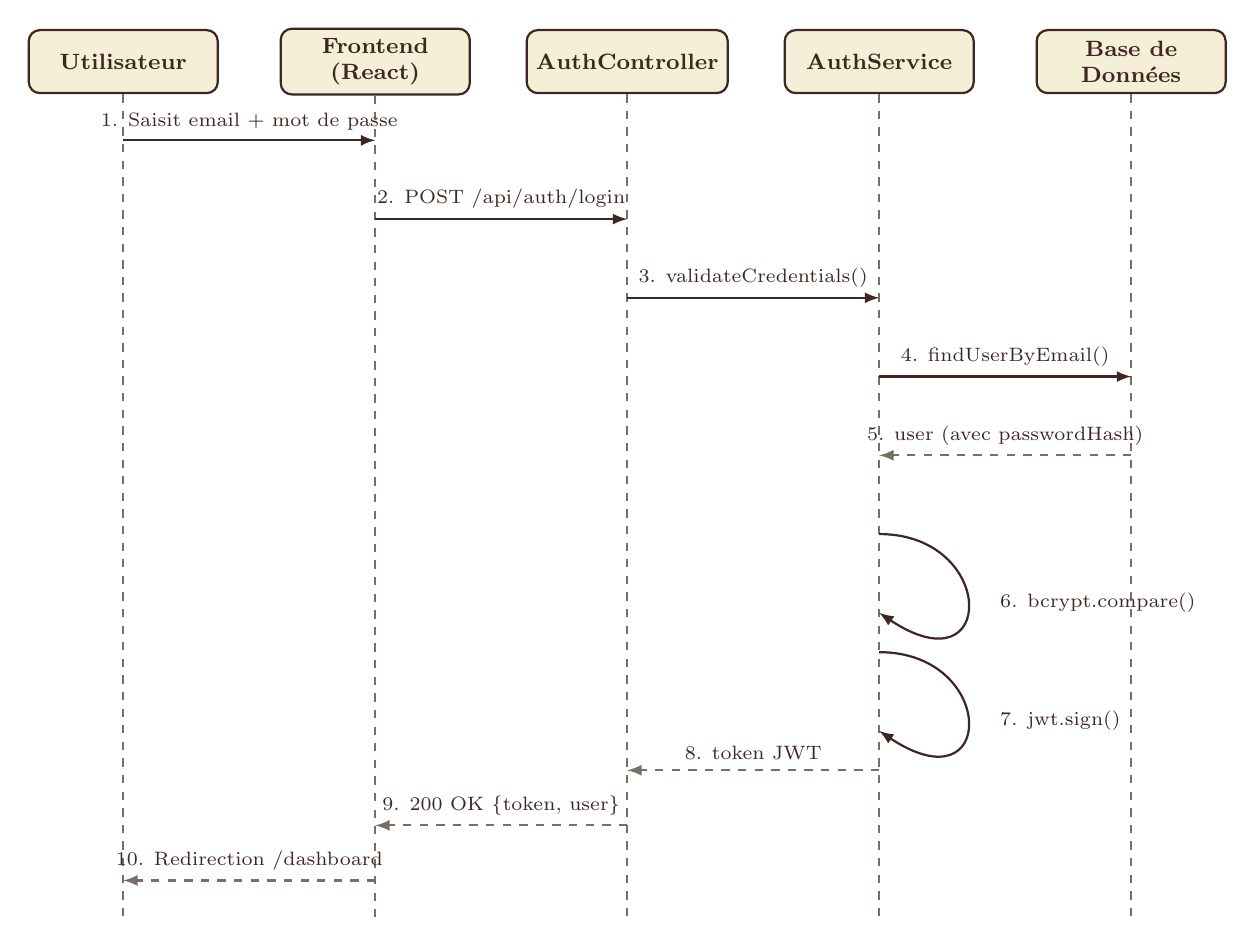
\begin{tikzpicture}[
    actor/.style={
        draw=SoftEspresso, thick, rounded corners=4pt,
        fill=GoldenGlow!20,
        minimum width=2.4cm, minimum height=0.8cm,
        font=\footnotesize\bfseries, text=SoftEspresso,
        align=center
    },
    lifeline/.style={
        dashed, thick, draw=AccentGray
    },
    activation/.style={
        draw=SoftEspresso, fill=GoldenGlow!40,
        minimum width=0.25cm
    },
    msg/.style={
        ->, >=latex, thick, draw=SoftEspresso
    },
    return/.style={
        ->, >=latex, thick, dashed, draw=AccentGray
    },
    msglabel/.style={
        font=\scriptsize, text=SoftEspresso,
        midway, above, sloped=false
    }
]

% ====== ACTEURS / OBJETS (en haut) ======
\node[actor] (user)  at ( 0,    0) {Utilisateur};
\node[actor] (front) at ( 3.2,  0) {Frontend\\(React)};
\node[actor] (ctrl)  at ( 6.4,  0) {AuthController};
\node[actor] (svc)   at ( 9.6,  0) {AuthService};
\node[actor] (db)    at (12.8,  0) {Base de\\Données};

% ====== LIGNES DE VIE ======
\foreach \n in {user, front, ctrl, svc, db}
    \draw[lifeline] (\n.south) -- ++(0, -10.5);

% ====== MESSAGES ======
% 1. Saisie identifiants
\draw[msg] (user.south |- 0,-1)  -- node[msglabel]{1. Saisit email + mot de passe} (front.south |- 0,-1);

% 2. POST /api/auth/login
\draw[msg] (front.south |- 0,-2) -- node[msglabel]{2. POST /api/auth/login} (ctrl.south |- 0,-2);

% 3. Validation
\draw[msg] (ctrl.south |- 0,-3)  -- node[msglabel]{3. validateCredentials()} (svc.south |- 0,-3);

% 4. Recherche utilisateur
\draw[msg] (svc.south |- 0,-4)   -- node[msglabel]{4. findUserByEmail()} (db.south |- 0,-4);

% 5. Retour user
\draw[return] (db.south |- 0,-5) -- node[msglabel]{5. user (avec passwordHash)} (svc.south |- 0,-5);

% 6. bcrypt.compare (auto-message)
\draw[msg] (svc.south |- 0,-6) .. controls +(1.5,0) and +(1.5,-1) ..
    node[right=8pt, font=\scriptsize, text=SoftEspresso]{6. bcrypt.compare()}
    (svc.south |- 0,-7);

% 7. Génération JWT (auto-message)
\draw[msg] (svc.south |- 0,-7.5) .. controls +(1.5,0) and +(1.5,-1) ..
    node[right=8pt, font=\scriptsize, text=SoftEspresso]{7. jwt.sign()}
    (svc.south |- 0,-8.5);

% 8. Retour token au controller
\draw[return] (svc.south |- 0,-9)  -- node[msglabel]{8. token JWT} (ctrl.south |- 0,-9);

% 9. Retour 200 + token au frontend
\draw[return] (ctrl.south |- 0,-9.7) -- node[msglabel]{9. 200 OK \{token, user\}} (front.south |- 0,-9.7);

% 10. Redirection dashboard
\draw[return] (front.south |- 0,-10.4) -- node[msglabel]{10. Redirection /dashboard} (user.south |- 0,-10.4);

\end{tikzpicture}
\caption{Diagramme de séquence -- Flux d'authentification (login)}
\label{fig:seq-login}
\end{figure}

\section{\color{SoftEspresso}Implémentation}
\subsection{\color{SoftEspresso}Authentification}
\begin{itemize}
    \item \textbf{\color{SoftEspresso}Hashing des mots de passe (bcrypt) :} La bibliothèque \texttt{bcrypt} est utilisée pour hacher les mots de passe avant de les stocker. C'est un algorithme adaptatif qui intègre un "sel" (\textit{salt}) pour se protéger contre les attaques par tables arc-en-ciel (\textit{rainbow tables}).
    \item \textbf{\color{SoftEspresso}JSON Web Tokens (JWT) :} Le flux d'authentification est basé sur les JWT. Un jeton est composé de trois parties : un en-tête, une charge utile (\textit{payload}) et une signature. La charge utile contient les informations de l'utilisateur (par exemple, \texttt{userId} et \texttt{role}), et la signature garantit l'intégrité du jeton.
\end{itemize}

\subsection{\color{SoftEspresso}Middleware de protection des routes}
Un middleware Express, nommé \texttt{protect}, est implémenté. Il effectue les actions suivantes pour chaque requête sur une route protégée :
\begin{enumerate}
    \item Extrait le JWT de l'en-tête \texttt{Authorization}.
    \item Vérifie la validité de la signature du jeton en utilisant une clé secrète.
    \item Si le jeton est valide, il décode la charge utile pour récupérer l'ID de l'utilisateur.
    \item Il récupère l'utilisateur correspondant dans la base de données et l'attache à l'objet de requête (\texttt{req.user}).
    \item Si une étape échoue, il renvoie une erreur 401 (Non autorisé).
\end{enumerate}

\subsection{\color{SoftEspresso}RBAC (Role-Based Access Control)}
Le contrôle d'accès basé sur les rôles est implémenté via un second middleware, \texttt{authorize(role)}. Ce middleware est utilisé après le middleware \texttt{protect}.
\begin{itemize}
    \item Il prend en paramètre le ou les rôles autorisés à accéder à la route.
    \item Il compare le rôle de l'utilisateur authentifié (\texttt{req.user.role}) avec les rôles autorisés.
    \item Si le rôle de l'utilisateur est dans la liste des rôles autorisés, la requête continue. Sinon, une erreur 403 (Interdit) est renvoyée.
\end{itemize}
\textbf{\color{SoftEspresso}Exemple :} La route de création d'un utilisateur (\texttt{POST /api/users}) serait protégée comme suit : \texttt{router.post('/', protect, authorize('ADMIN'), userController.createUser)}. Seul un administrateur authentifié peut y accéder.

\section{\color{SoftEspresso}Sécurité}
Plusieurs mesures de sécurité ont été intégrées pour renforcer le module :
\begin{itemize}
    \item \textbf{\color{SoftEspresso}Hashing des mots de passe :} Utilisation de \texttt{bcrypt} avec un coût de calcul (\textit{cost factor}) de 12 pour ralentir les attaques par force brute.
    \item \textbf{\color{SoftEspresso}Expiration des jetons :} Les JWT ont une durée de vie limitée (par exemple, 1 heure pour les jetons d'accès) pour réduire la fenêtre d'opportunité en cas de vol de jeton. Un mécanisme de rafraîchissement de jeton (\textit{refresh token}) est utilisé pour maintenir la session utilisateur.
    \item \textbf{\color{SoftEspresso}Limitation de débit :} Le middleware \texttt{express-rate-limit} est configuré pour limiter le nombre de tentatives de connexion à partir d'une même adresse IP, atténuant ainsi les attaques par force brute.
    \item \textbf{\color{SoftEspresso}Gestion des erreurs :} Les messages d'erreur sont génériques (par exemple, "Email ou mot de passe invalide") pour ne pas révéler si un email existe ou non dans la base de données.
    \item \textbf{\color{SoftEspresso}Validation des entrées :} La bibliothèque \texttt{express-validator} est utilisée pour valider et assainir toutes les données entrantes du client afin de prévenir les attaques par injection (par exemple, XSS).
\end{itemize}

\section{\color{SoftEspresso}Intégration Frontend}
Côté frontend (React), l'intégration se manifeste par :
\begin{itemize}
    \item \textbf{\color{SoftEspresso}Page de connexion :} Un formulaire contrôlé qui envoie les identifiants à l'API et gère les réponses (succès ou erreur).
    \item \textbf{\color{SoftEspresso}Routes protégées :} Utilisation de \texttt{react-router} pour créer des composants de route privée qui vérifient la présence d'un jeton d'authentification valide avant d'afficher une page. Si l'utilisateur n'est pas authentifié, il est redirigé vers la page de connexion.
    \item \textbf{\color{SoftEspresso}Interface utilisateur basée sur les rôles :} Le frontend adapte les éléments d'interface affichés en fonction du rôle de l'utilisateur, stocké dans le contexte de l'application. Par exemple, un bouton "Panneau d'administration" ne sera visible que si l'utilisateur a le rôle \texttt{ADMIN}.
\end{itemize}

% ════════════════════════════════════════════════════════════
% NOUVELLE SECTION : CAPTURES D'ECRAN
% ════════════════════════════════════════════════════════════
\section{\color{SoftEspresso}Captures d'écran de l'Application}

Cette section présente les principales interfaces du module
d'authentification et de gestion des rôles, telles qu'elles apparaissent
à l'utilisateur final.

% ────────────────────────────────────────────────────────────
\subsection{\color{SoftEspresso}Page de Connexion}

La figure \ref{fig:login} présente la page de connexion principale,
accessible à tous les utilisateurs (admin, enseignant, étudiant).
L'utilisateur saisit son adresse e-mail et son mot de passe, puis le
système valide ses identifiants côté serveur.

\begin{figure}[H]
    \centering
    \includegraphics[width=0.85\textwidth]{login.png}
    \caption{Page de connexion à la plateforme SGUI}
    \label{fig:login}
\end{figure}

% ────────────────────────────────────────────────────────────
\subsection{\color{SoftEspresso}Erreur de Connexion (Identifiants Invalides)}

Lorsque les identifiants saisis sont incorrects, un message d'erreur
générique est affiché afin de ne pas révéler si l'email existe ou non
dans la base de données.

\begin{figure}[H]
    \centering
    \includegraphics[width=0.85\textwidth]{login-error.png}
    \caption{Affichage du message d'erreur en cas d'échec d'authentification}
    \label{fig:login-error}
\end{figure}

% ────────────────────────────────────────────────────────────
\subsection{\color{SoftEspresso}Création d'un Compte Utilisateur (Admin)}

La création de comptes est une fonctionnalité réservée à l'administrateur.
La figure \ref{fig:create-user} montre le formulaire permettant à l'admin
d'ajouter un nouvel utilisateur en spécifiant son rôle (admin, enseignant
ou étudiant).

\begin{figure}[H]
    \centering
    \includegraphics[width=0.85\textwidth]{create-user.png}
    \caption{Formulaire de création d'un compte utilisateur (interface admin)}
    \label{fig:create-user}
\end{figure}

% ────────────────────────────────────────────────────────────
\subsection{\color{SoftEspresso}Gestion des Utilisateurs (Liste Admin)}

L'administrateur peut consulter la liste complète des utilisateurs
enregistrés, filtrer par rôle, modifier ou désactiver un compte.

\begin{figure}[H]
    \centering
    \includegraphics[width=0.95\textwidth]{users-list.png}
    \caption{Liste des utilisateurs avec actions de gestion (admin)}
    \label{fig:users-list}
\end{figure}

% ────────────────────────────────────────────────────────────
\subsection{\color{SoftEspresso}Changement de Mot de Passe}

Tout utilisateur authentifié peut modifier son mot de passe depuis son
profil. Le système exige la saisie du mot de passe actuel pour des
raisons de sécurité, puis applique un hachage bcrypt au nouveau mot de
passe avant de le stocker.

\begin{figure}[H]
    \centering
    \includegraphics[width=0.85\textwidth]{change-password.png}
    \caption{Formulaire de changement de mot de passe}
    \label{fig:change-password}
\end{figure}

% ────────────────────────────────────────────────────────────
\subsection{\color{SoftEspresso}Tableaux de Bord par Rôle}

L'interface s'adapte automatiquement au rôle de l'utilisateur connecté.
Chaque profil dispose d'un tableau de bord spécifique présentant les
fonctionnalités auxquelles il a accès.

\begin{figure}[H]
    \centering
    \includegraphics[width=0.95\textwidth]{dashboard-admin.png}
    \caption{Tableau de bord de l'administrateur}
    \label{fig:dashboard-admin}
\end{figure}

\begin{figure}[H]
    \centering
    \includegraphics[width=0.95\textwidth]{dashboard-teacher.png}
    \caption{Tableau de bord de l'enseignant}
    \label{fig:dashboard-teacher}
\end{figure}

\begin{figure}[H]
    \centering
    \includegraphics[width=0.95\textwidth]{dashboard-student.png}
    \caption{Tableau de bord de l'étudiant}
    \label{fig:dashboard-student}
\end{figure}

% ────────────────────────────────────────────────────────────
\subsection{\color{SoftEspresso}Profil Utilisateur}

Chaque utilisateur authentifié peut consulter et mettre à jour les
informations de son profil personnel.

\begin{figure}[H]
    \centering
    \includegraphics[width=0.85\textwidth]{profile.png}
    \caption{Page de profil utilisateur}
    \label{fig:profile}
\end{figure}

% ════════════════════════════════════════════════════════════
% FIN NOUVELLE SECTION
% ════════════════════════════════════════════════════════════

\section{\color{SoftEspresso}Tests et Validation}
Des tests ont été menés pour valider le bon fonctionnement et la sécurité du module :
\begin{itemize}
    \item \textbf{\color{SoftEspresso}Tests de connexion :} Vérification des scénarios de connexion réussie et échouée.
    \item \textbf{\color{SoftEspresso}Tests d'accès non autorisé :} Tentatives d'accès à des routes protégées sans jeton ou avec un jeton invalide, s'assurant qu'une erreur 401 est bien retournée.
    \item \textbf{\color{SoftEspresso}Tests des rôles :} Tentatives d'accès à des routes restreintes par un utilisateur authentifié mais avec un rôle insuffisant (par exemple, un étudiant essayant d'accéder à une ressource d'administration), s'assurant qu'une erreur 403 est retournée.
\end{itemize}

\section{\color{SoftEspresso}Résultats}
Les tests ont confirmé que le système d'authentification et de gestion des rôles est fonctionnel, sécurisé et stable. Les objectifs fixés ont été atteints : l'accès à la plateforme est contrôlé, les utilisateurs sont identifiés de manière fiable et les permissions sont appliquées correctement en fonction des rôles, garantissant une séparation claire des responsabilités au sein de l'application.

\end{document}
